%!TEX root = ../../14-icra-RealTimeNMPC.tex

\tikzstyle{block} = [draw, fill=blue!20, rectangle,
    minimum height=2em, minimum width=5em, align=center]
\tikzstyle{sum} = [draw, fill=blue!20, circle, node distance=1cm]
\tikzstyle{input} = [coordinate]
\tikzstyle{output} = [coordinate]
\tikzstyle{pinstyle} = [pin edge={to-,thin,black}]

% The block diagram code is probably more verbose than necessary
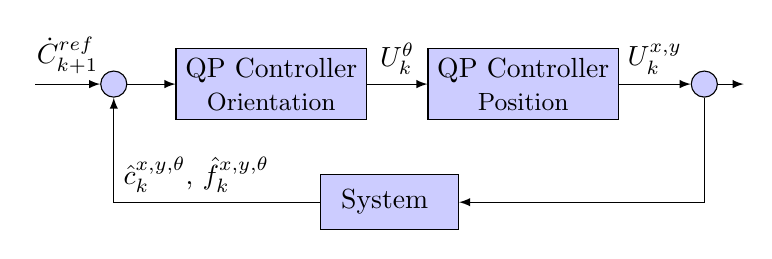
\begin{tikzpicture}[auto, node distance=2cm,>=latex]
    % We start by placing the blocks
    \node [input]  at (-1, 0.0) (input)  {};
    \node [sum]    at ( 0.0, 0.0) (sumin)  {};
    \node [sum]    at ( 7.5, 0.0) (sumout) {};
    \node [output] at ( 8.0, 0.0) (output) {};

    % QP Controller Blocks
    \node [block] at (2,0) (oriqp) {
        QP Controller \\
        \small{Orientation}
    };
    \node [block] at (5.2,0) (posqp) {
        QP Controller \\
        \small{Position}
    };
    \node [block] at (3.5, -1.5) (system) {
    		System
    	};

    % PATHS
	% Forward chaine
    \draw [draw,->] (input) -- node {$
        \dot C_{k+1}^{ref}
    $} (sumin);
    \draw [->] (sumin) -- node {} (oriqp);
    \draw [->] (oriqp) -- node {$U_k^{\theta}$} (posqp);
    \draw [->] (posqp) -- node {$U_k^{x,y}$} (sumout);
    \draw [->] (sumout) -- node {} (output);

    % Feedback chaine
    \draw [->] (sumout) |- node {} (system);
    \draw [->] (system) -| node[above right] {$\hat{c}_k^{x,y,\theta}$, $\hat{f}_k^{x,y,\theta}$} (sumin);
\end{tikzpicture}


% The block diagram code is probably more verbose than necessary
%\begin{tikzpicture}[auto, node distance=2cm,>=latex']
%    % We start by placing the blocks
%    \node [input]  at (-0.5, 0.0) (input)  {};
%    \node [sum]    at ( 0.5, 0.0) (sumin)  {};
%    \node [sum]    at ( 6.5, 0.0) (sumout) {};
%    \node [output] at ( 7.5, 0.0) (output) {};
%
%    % QP Controller Blocks
%    \node [block] at (2.0,0) (oriqp) {
%        QP Controller\\
%        \small{Orientation}
%    };
%    \node [block] at (5.0,0) (posqp) {
%        QP Controller\\
%        \small{Position}
%    };
%    \node [block] at (5.0, -2.0) (dynamics) {Dynamics};
%    \node [block] at (2.0, -2.0) (system)   {System};
%
%    % PATHS
%    \draw [draw,->] (input) -- node {$
%        \dot C_{k+1}^{ref}
%    $} (sumin);
%    \draw [->] (oriqp) -- node {$U_k$} (posqp);
%    \draw [->] (posqp) -- node {$U_k$} (sumout);
%    \draw [->] (dynamics) --  (system);
%
%    \draw [->] (sumout) -- node {$ $} (output);
%    \draw [->] (sumin) -- node {} (oriqp);
%    \draw [->] (sumout) |- node[near start] {$y$}   (dynamics);
%    \draw [->] (system) -| node[near end]   {$val$} (sumin);
%\end{tikzpicture}
